\documentclass[12pt, twoside]{article}
\input{../preamble}
\usepackage{float}

\fancyhead[LO]{La Scuola d'Italia / Dr.\ Huson / IB Math \\* 20 May 2026}
\fancyhead[RO]{\fbox{\begin{minipage}{6cm}\footnotesize First \& Last name:\\[0.5cm]\end{minipage}}}
\fancyfoot[C]{\thepage}

\begin{document}
\subsubsection*{8.2 Classwork: Rational Functions --- Toward the Maturit\`a}

\begin{enumerate}[itemsep=0.4cm]

%--- Problem 1: Standard form (ax+b)/(cx+d) review ---
\item[1.] Consider $\displaystyle f(x)=\dfrac{x+3}{x-2}$.

\begin{enumerate}[label=(\alph*), itemsep=0.3cm]
  \item State the equation of the vertical asymptote.

  \vspace{1.2cm}

  \item Verify by long division (or otherwise) that
  $\displaystyle f(x)=1+\dfrac{5}{x-2}$.
  Use this form to state the equation of the horizontal asymptote.

  \vspace{2.4cm}

  \item Find the $x$-intercept and the $y$-intercept.

  \vspace{2.7cm}

  \item Sketch $f$ on the axes below. Mark and label the asymptotes and intercepts.
\end{enumerate}

\begin{figure}[H]
\begin{center}
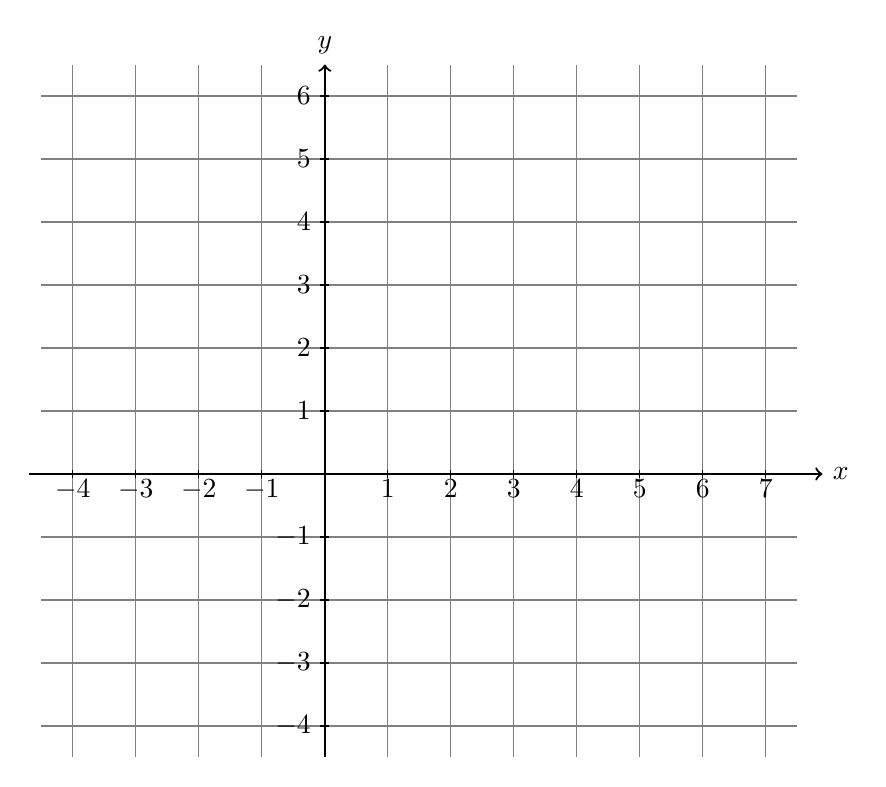
\begin{tikzpicture}[scale=0.8]

\draw [thin, color=gray, xstep=1.0cm, ystep=1.0cm] (-4.5,-4.5) grid (7.5,6.5);

\foreach \x in {-4,-3,-2,-1,1,2,3,4,5,6,7}
\draw[shift={(\x,0)}, color=black] (0pt,-2pt) -- (0pt,2pt) node[below] {$\x$};

\foreach \y in {-4,-3,-2,-1,1,2,3,4,5,6}
\draw[shift={(0,\y)}, color=black] (2pt,0pt) -- (-2pt,0pt) node[left] {$\y$};

\draw [thick, ->] (-4.7,0) -- (7.9,0) node [right] {$x$};
\draw [thick, ->] (0,-4.5) -- (0,6.5) node [above] {$y$};

\end{tikzpicture}
\end{center}
\end{figure}

\newpage

%--- Problem 2: Family (x-2)/(x-a) with parameter ---
\item[2.] Consider the family of functions
$\displaystyle f_a(x)=\dfrac{x-2}{x-a}$, with $a\ne 2$.

\begin{enumerate}[label=(\alph*), itemsep=0.3cm]
  \item For an arbitrary value of $a$, state the equation of the
  vertical asymptote of $f_a$.

  \vspace{1.2cm}

  \item Find the horizontal asymptote of $f_a$. Does its equation
  depend on $a$?

  \vspace{1.8cm}

  \item Compute $f_a(2)$. What does this tell you about a point
  shared by every curve in the family?

  \vspace{2.5cm}

  \item Now set $a=-1$. Find the $y$-intercept of $f_{-1}$ and
  sketch its graph on the axes below. Mark the asymptotes
  (dashed) and the intercepts.
\end{enumerate}

\begin{figure}[H]
\begin{center}
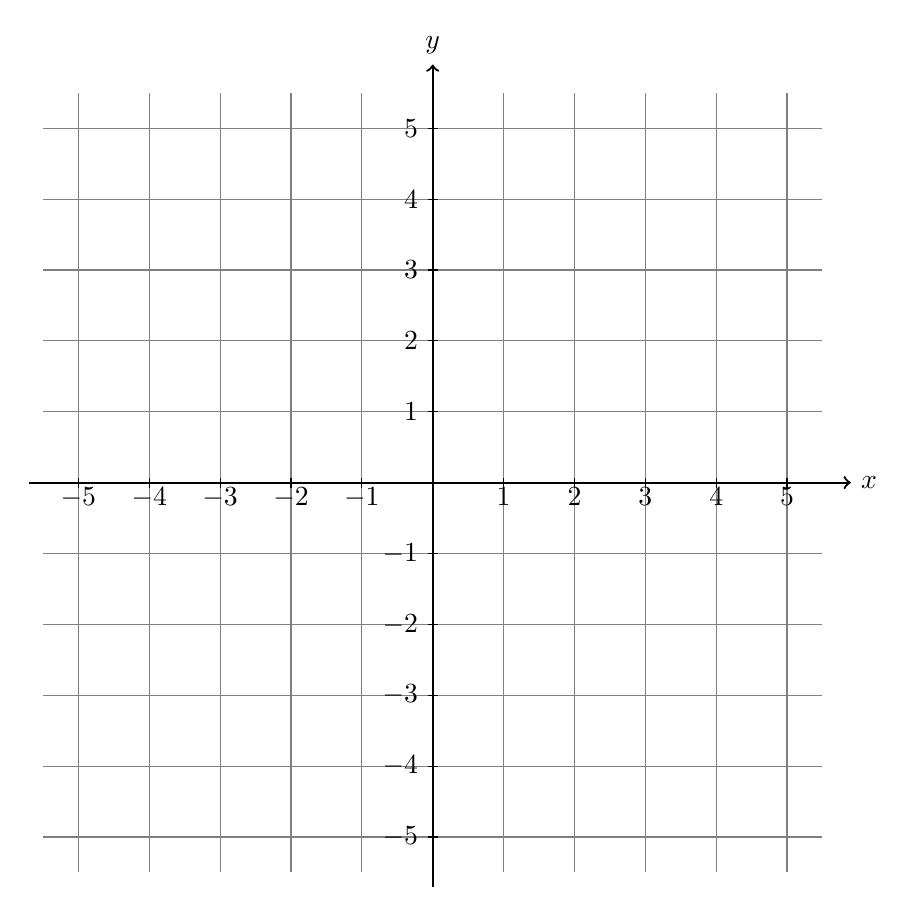
\begin{tikzpicture}[scale=0.9]

\draw [thin, color=gray, xstep=1.0cm, ystep=1.0cm] (-5.5,-5.5) grid (5.5,5.5);

\foreach \x in {-5,-4,-3,-2,-1,1,2,3,4,5}
\draw[shift={(\x,0)}, color=black] (0pt,-2pt) -- (0pt,2pt) node[below] {$\x$};

\foreach \y in {-5,-4,-3,-2,-1,1,2,3,4,5}
\draw[shift={(0,\y)}, color=black] (2pt,0pt) -- (-2pt,0pt) node[left] {$\y$};

\draw [thick, ->] (-5.7,0) -- (5.9,0) node [right] {$x$};
\draw [thick, ->] (0,-5.7) -- (0,5.9) node [above] {$y$};

\end{tikzpicture}
\end{center}
\end{figure}

\newpage

%--- Problem 3: Specific rational function with no VA ---
\item[3.] Consider $\displaystyle g(x)=\dfrac{x^2+x}{x^2+1}$.

\begin{enumerate}[label=(\alph*), itemsep=0.3cm]
  \item State the domain of $g$. (Hint: look at the denominator
  carefully --- can it equal zero?)

  \vspace{1.6cm}

  \item Compute $\displaystyle\lim_{x\to+\infty}g(x)$ and
  $\displaystyle\lim_{x\to-\infty}g(x)$. Hence state the
  horizontal asymptote.

  \vspace{2.2cm}

  \item Find the $x$-intercepts (note: there are two) and the
  $y$-intercept.

  \vspace{2.6cm}

  \item Complete the table of values, then sketch the graph
  below.
\end{enumerate}

\vspace{0.2cm}
\begin{center}
\renewcommand{\arraystretch}{1.6}
\begin{tabular}{|c|c|c|c|c|c|c|c|c|}
\hline
$x$    & $-3$ & $-2$ & $-1$ & $0$ & $1$ & $2$ & $3$ & $5$ \\
\hline
$g(x)$ & \phantom{XXXX} & \phantom{XXXX} & \phantom{XXXX} & \phantom{XXXX} & \phantom{XXXX} & \phantom{XXXX} & \phantom{XXXX} & \phantom{XXXX} \\
\hline
\end{tabular}
\end{center}

\begin{figure}[H]
\begin{center}
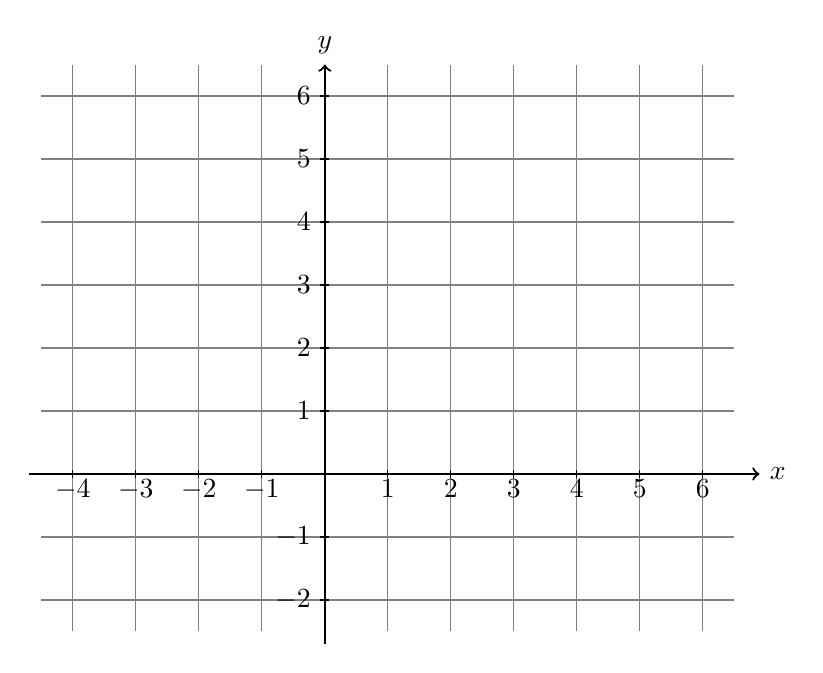
\begin{tikzpicture}[scale=0.8]

\draw [thin, color=gray, xstep=1.0cm, ystep=1.0cm] (-4.5,-2.5) grid (6.5,6.5);

\foreach \x in {-4,-3,-2,-1,1,2,3,4,5,6}
\draw[shift={(\x,0)}, color=black] (0pt,-2pt) -- (0pt,2pt) node[below] {$\x$};

\foreach \y in {-2,-1,1,2,3, 4, 5,6}
\draw[shift={(0,\y)}, color=black] (2pt,0pt) -- (-2pt,0pt) node[left] {$\y$};

\draw [thick, ->] (-4.7,0) -- (6.9,0) node [right] {$x$};
\draw [thick, ->] (0,-2.7) -- (0,6.5) node [above] {$y$};

\end{tikzpicture}
\end{center}
\end{figure}

\newpage

%--- Problem 4: Family (x^2 - ax)/(x^2 - a) — domain and HA crossings ---
\item[4.] Consider the family of functions
$\displaystyle f_a(x)=\dfrac{x^2-ax}{x^2-a}$, with $a\ne 0$.

The function $g$ from Problem 3 is the member $f_{-1}$
(check: substituting $a=-1$ gives $g(x)=(x^2+x)/(x^2+1)$).

\begin{enumerate}[label=(\alph*), itemsep=0.3cm]
  \item Find the domain of $f_a$ in each of the following cases.

  \vspace{0.2cm}

  \quad (i) $a<0$ (for example $a=-1$, $a=-3$):
  \vspace{1.0cm}

  \quad (ii) $a>0$ (for example $a=4$):
  \vspace{1.0cm}

  \item State the equation of the horizontal asymptote of $f_a$.
  (Hint: same idea as Problem 3(b) --- compare leading terms.)

  \vspace{1.6cm}

  \item Set $f_a(x)$ equal to the horizontal asymptote you found in
  (b), and solve for $x$. Show that the solution does not depend
  on $a$ (provided $a\ne 1$). Conclude that every curve $\Omega_a$
  in the family passes through one common point on its horizontal
  asymptote. State this point.

  \vspace{4.5cm}

  \item Compute $f_a(0)$. Then show, using the quotient rule, that
  $f_a'(0)=1$ for every $a\ne 0$. Hence write down the equation
  of the line tangent to $\Omega_a$ at the origin. Is this line
  the same for every $a$?

  \vspace{4cm}
\end{enumerate}

\newpage

%--- Problem 5: Oblique asymptote — (x^3 + 4)/x^2 ---
\item[5.] Consider $\displaystyle h(x)=\dfrac{x^3+4}{x^2}$.

\begin{enumerate}[label=(\alph*), itemsep=0.25cm]
  \item State the domain of $h$, and the equation of the vertical
  asymptote.

  \vspace{0.5cm}

  \item Show that $\displaystyle h(x)=x+\dfrac{4}{x^2}$.

  \vspace{1.8cm}

  \item Use part (b) to explain why the graph of $h$ approaches
  the line $y=x$ as $|x|$ grows large. This line is called the
  \emph{oblique asymptote} of $h$.

  \vspace{1.6cm}

  \item Complete the table of values for $h$.
  \vspace{0.1cm}
  \begin{center}
  \renewcommand{\arraystretch}{1.4}
  \begin{tabular}{|c|c|c|c|c|c|c|c|c|}
  \hline
  $x$    & $-3$ & $-2$ & $-1$ & $-0.5$ & $0.5$ & $1$ & $2$ & $4$ \\
  \hline
  $h(x)$ & \phantom{XXX} & \phantom{XXX} & \phantom{XXX} & \phantom{XXX} & \phantom{XXX} & \phantom{XXX} & \phantom{XXX} & \phantom{XXX} \\
  \hline
  \end{tabular}
  \end{center}

  \item Sketch the graph on the axes below. Show both the vertical
  asymptote and the oblique asymptote $y=x$ as dashed lines.
\end{enumerate}

\begin{figure}[H]
\begin{center}
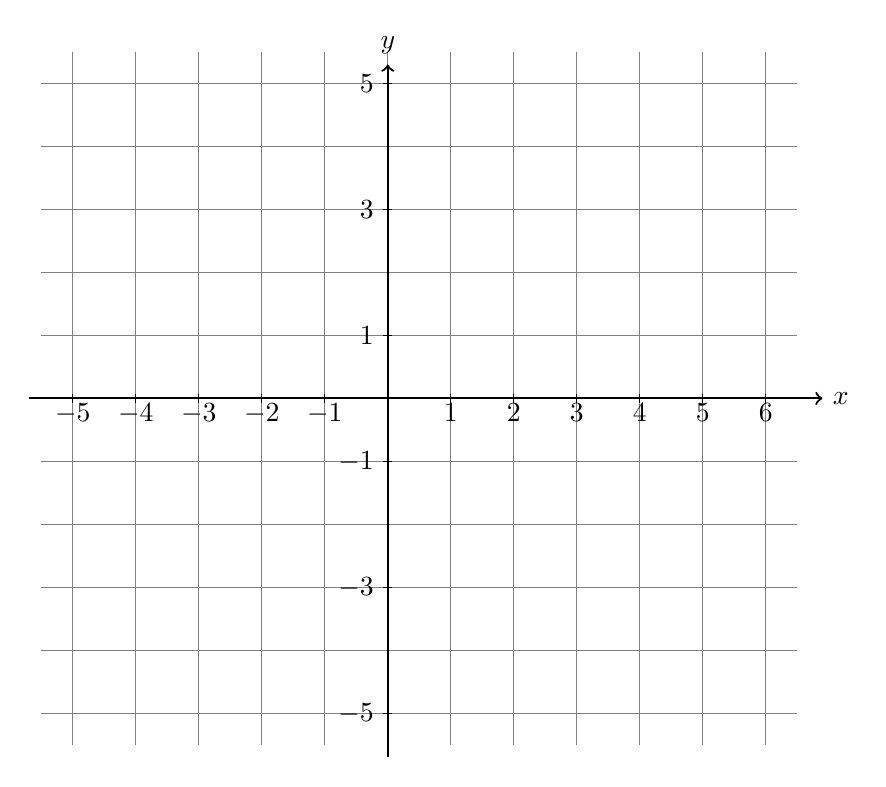
\begin{tikzpicture}[scale=0.8]

\draw [thin, color=gray, xstep=1.0cm, ystep=1.0cm] (-5.5,-5.5) grid (6.5,5.5);

\foreach \x in {-5,-4,-3,-2,-1,1,2,3,4,5,6}
\draw[shift={(\x,0)}, color=black] (0pt,-2pt) -- (0pt,2pt) node[below] {$\x$};

\foreach \y in {-5,-3,-1,1,3,5}
\draw[shift={(0,\y)}, color=black] (2pt,0pt) -- (-2pt,0pt) node[left] {$\y$};

\draw [thick, ->] (-5.7,0) -- (6.9,0) node [right] {$x$};
\draw [thick, ->] (0,-5.7) -- (0,5.3) node [above] {$y$};

\end{tikzpicture}
\end{center}
\end{figure}

\newpage

%--- Page 6: Maturita problems in Italian (no answer space) ---
\begin{center}
\textbf{\large Problemi della Maturit\`a} \\[2pt]
\small (Use separate paper for these problems.)
\end{center}

\vspace{0.4cm}

\item[6.] \textbf{PROBLEMA 2 --- Sessione ordinaria 2023.}

Fissato un parametro reale $a$, con $a\ne 0$, si consideri la
funzione $f_a$ cos\`i definita:
$$f_a(x)=\dfrac{x^2-ax}{x^2-a}$$
il cui grafico sar\`a indicato con $\Omega_a$.

\begin{enumerate}[label=(\alph*), itemsep=0.25cm]
  \item Al variare del parametro $a$, determinare il dominio di
  $f_a$, studiarne le eventuali discontinuit\`a e scrivere le
  equazioni di tutti i suoi asintoti.

  \item Mostrare che, per $a\ne 1$, tutti i grafici $\Omega_a$
  intersecano il proprio asintoto orizzontale in uno stesso
  punto e condividono la stessa retta tangente nell'origine.
\end{enumerate}

\vspace{0.6cm}

\item[7.] \textbf{PROBLEMA 1 --- Sessione ordinaria 2024.}

Si consideri $\displaystyle f_{a,b}(x)=\dfrac{ax^3+b}{x^2}$, con
$a,b\in\mathbb{R}$.

\begin{enumerate}[label=(\alph*), itemsep=0.25cm]
  \item Determinare i valori dei parametri in modo che la retta
  $t$, di equazione $7x+y-12=0$, sia tangente al grafico di
  $f_{a,b}(x)$ nel suo punto $P$ di ascissa $x=1$.

  \medskip
  Si ponga, d'ora in avanti, $a=1$ e $b=4$.

  \item Studiare la funzione $\displaystyle f(x)=\dfrac{x^3+4}{x^2}$
  e tracciarne il grafico $\gamma$.
\end{enumerate}

\end{enumerate}
\end{document}
